\subsection{IrDA* Port}
\label{sec:irda_port}

The \systemName~includes an IrDA UART for communicating wirelessly with peripherals over 
the infrared spectrum. It is configured for 8-bit data and one stop bit, and operates at a baud 
rate of 155,200. The default configuration does not use a parity bit. The programming interface 
consists of two 32-bit registers, as shown in Figure~\ref{fig:irda_port}. The register at 
address {\sf 0xFF201020} is referred to as the {\it Data} register, and the register at 
address {\sf 0xFF201024} is the {\it Control} register. 

The operation of the IrDA UART is similar to the Serial Port UART described above. Data recieved 
through the IrDA is stored in a 128-character FIFO in the UART. As shown in 
Figure~\ref{fig:irda_port}, the number of characters, {\it RAVAIL}, currently stored in this FIFO 
is provided in bits 23$-$16 of the {\it Data} register. If the FIFO overflows, then any 
additional data is lost. When a read of the {\it Data} register is performed, the character
at the head of the FIFO is provided in bits 7$-$0. If the character read is valid, the the value 
of bit 15, {\it RVALID} will be one. If no data is available to be read from the receive FIFO, 
then {\it RVALID} will be set to 0 and the data in bits $7-0$ is undefined. 

\begin{figure}[h!]
   \begin{center}
       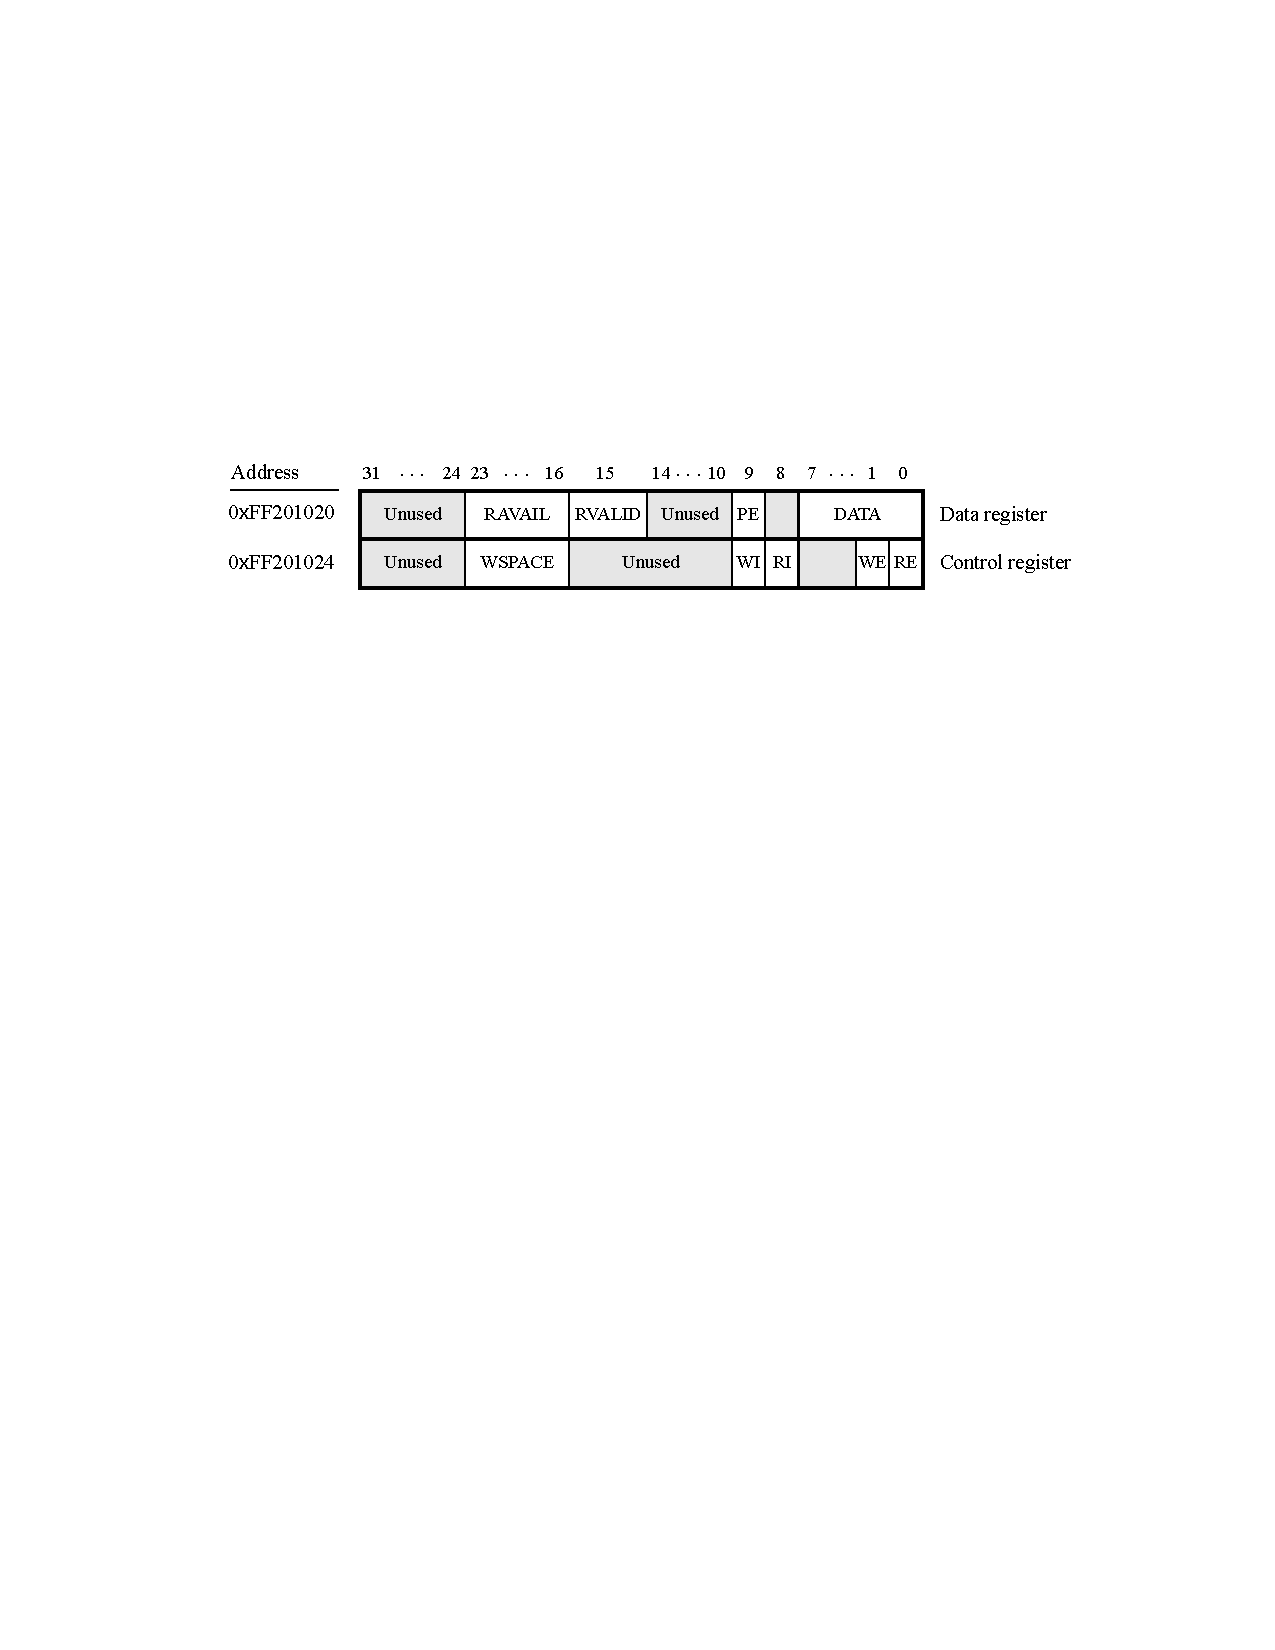
\includegraphics{../../../common/figs/Media_FPGA_IrDA.pdf}
   \end{center}
   \caption{IrDA UART registers.}
	\label{fig:irda_port}
\end{figure}

The {\it Control} register bits {\it RE} and {\it RI} are described in section \ref{sec:exceptions}.